%%%%%%%%%%%%
%PAGE SETUP%
%%%%%%%%%%%%
\documentclass[letterpaper,11pt]{article}
\usepackage[margin=1.0in]{geometry}
%empty header/footers; i.e. don't number pages
\thispagestyle{empty}


%%%%%%%%%
%IMPORTS%
%%%%%%%%%

\usepackage{titlesec}
\usepackage[usenames,dvipsnames]{color}
\usepackage[pdftex]{hyperref}
\usepackage{enumitem}
\usepackage{listings}

\usepackage{graphicx}
\graphicspath{{./Images/}}

\usepackage[T1]{fontenc}

%%%%%%
%MISC%
%%%%%%
\newcommand{\myLink}[2]{\href{#1}{\color{blue}\underline{\smash{\texttt{#2}}}}}
\newcommand{\myURL}[1]{\myLink{https://#1}{#1}}

\title{CS 431: Weight Scale Project}
\author{Ivan Johnson \and Soham Karanjikar}
\date{2020-05-01}

\pagestyle{empty}


%%%%%%%
%BEGIN%
%%%%%%%
\begin{document}

\maketitle

\newpage
\section{Introduction}
The main objective of this project was to create a weight scale and display the
readings somewhere visible. The requirement was to use some sort of micro
controller and apply the concept we had learned in CS 431 to a practical,
useful, example. The initial plan was to use an existing scale and try to take
readings through communicating with the micro controller on the scale, however,
this proved to be more work than creating a new scale. The components,
procedure, results and future possibilities are explained in this paper.

In the appendices we reproduce our original proposal, a listing of our exact
code, and a list of what we used for this project.

\section{Components}
\subsection{Micro-controller}
The board used was an Arduino Uno, a hobbyist development board used in many
projects at their preliminary stage, with the MCU being an ATMEGA4809. The
reason for choosing this board was because of the ease of using it and the
libraries already available for communicating with various chips. Further, the
Arduino IDE is also very user friendly and allowed us to quickly test code.

We could have potentially used a cheaper and smaller option such as an ESP32,
but there were Arduinos already present in the lab which allowed us to start
immediately.

\subsection{Load Cells and Amplifier Chip}
While researching methods to communicate with a controller on an existing scale
we found that load cells and their controller chip are very cheap and easy to
use. This is the reason we decided to build our own scale rather than tapping
into a pre-made scale.

The chip used for reading values from load cells is the HX711, an amplifier chip
specifically designed for load cells.

The bundle purchased came with 4 load cells included in it. These load cells had
an individual rating of 50Kg each allowing us to make a scale that could provide
accurate readings of masses up to 200Kg. The load cells were generic and came
with no model/serial number or brand.

\section{Procedure}
\subsection{Wiring}
Load cells use strain gauges to measure weight. A strain gauge contains a wire
carefully shaped such that its resistance varies when the strain gauge undergoes
elastic deformation. To form the load cell, the strain gauge is attached to a
piece of metal in such a way that the strain gauge can be used to measure the
deformation of the metal and infer the force that is being applied to the load
cell.

The load cells are wired according to the specification given to use in a
Wheatstone Bridge configuration, as shown in figure \ref{img:banggood}.

\begin{figure}[h]
  \centering
  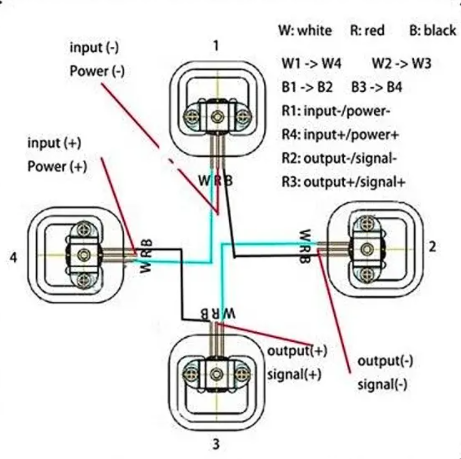
\includegraphics[scale=.5]{loadcellwiring}
  \caption{Image obtained from
    \myLink{https://www.banggood.com/4pcs-DIY-50KG-Body-Load-Cell-Weight-Strain-Sensor-Resistance-With-HX711-AD-Module-p-1326815.html}{Bang
      Good}}
  \label{img:banggood}
\end{figure}

Since the change in resistance is quite small, we use an amplifier chip, the
HX711. This chip also has ADC included in it which allows us to directly
communicate with it using the serial protocol given in the documentation. The
whole systems wiring diagram is provided in figure \ref{img:wiring}.

\begin{figure}[h]
  \centering
  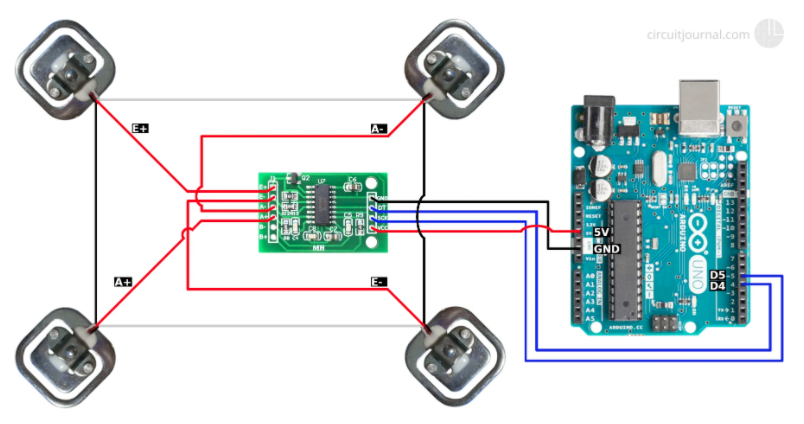
\includegraphics[scale=.3]{sytemwiring}
  \caption{Image obtained from
    \myLink{https://circuitjournal.com/50kg-load-cells-with-HX711}{Circuit Journal}}
  \label{img:wiring}
\end{figure}

The Arduino uses its 5V out to power the HX711 chip and 2 GPIOs to handle the
communication, 1 for clock and 1 for data.

\subsection{Software}
All the code was written in the Arduino IDE as a sketch; the code is available
in section \ref{apx:code} of the appendix. We only had one external dependency,
a \myLink{https://github.com/bogde/HX711}{HX711 library}. This library allowed
us to communicate with the amplifier chip quite easily as the low level
communication was already written for us. Figure \ref{img:stateflow} shows a
state diagram of our software.

\begin{figure}[h]
  \centering
  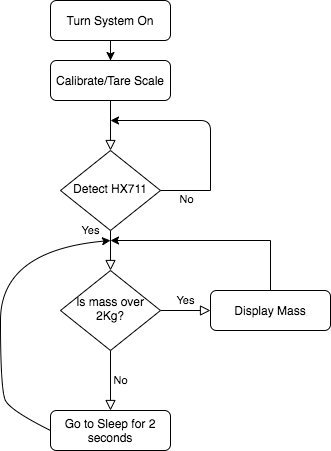
\includegraphics[scale=.7]{Flow}
  \caption{The state diagram of our code}
  \label{img:stateflow}
\end{figure}

The detection of HX711 is done by using the "is\_ready()" function from the
library which just checks if there is valid communication. Then the system
starts polling to read values from the chip, if they are above a certain
threshold (2Kg in our case) then the value is displayed on the console. If the
reading is not above that threshold then the system goes to sleep by turning the
CPU to its lowest sleep state and the HX711 to the sleep state. This allows for
a lot of power saving as most of the time the scale is not used.

The sleep mode used is the "Power Down Mode" which is the lowest power
consumption state of the MCU. The sleep modes and their power consummations are
shown in figure \ref{img:sleep}

\begin{figure}[h]
  \centering
  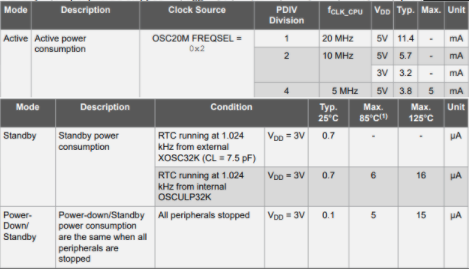
\includegraphics[width=1.0\textwidth]{powermodes}
  \caption{Image obtained from \myLink{http://ww1.microchip.com/downloads/en/DeviceDoc/ATmega4808-4809-Data-Sheet-DS40002173A.pdf}{ATMEGA 4809 Datasheet}}
  \label{img:sleep}
\end{figure}

By putting the MCU to sleep we save 10\textsuperscript{3}W of power as the
current consumption goes from mA to uA.

The only way to wake up from this sleep mode is using an external pin interrupt
or an Real Time Clock Interrupt. We would have liked to used an external
interrupt that triggered only when there is a mass above 2Kg on the scale,
however, the digital communication did not allow us to do that. Instead we had
to use the on board RTC to send a periodic interrupt to the MCU every 2 seconds
to wake it up and check the mass. This is the best we could do to keep the
process of reading autonomous (not turning the scale off and on every time using
a switch).


\subsection{Problems Encountered}

There were not many issues faced during the initial build of the system as
everything was documented well, the process just took time to learn how to use
the library and set up the hardware. The problems occurred after we had to move
away from campus due to COVID-19 and did not have access to the Arduino we were
using as it belonged to the lab. We had to switch to a new Arduino board that
did not support the same sleep modes available. This process was tedious as a
lot of testing had to be done to figure out how to use the RTC to wake up the
MCU. In the end we did figure it out. Further, working on the project when the
team had to communicate online was also difficult as only one of us could see
the errors firsthand.

Another problem was that the scale's calibration value had to be reset after
physically moving the scale anytime. This was due to the fact that the slightest
movement of the load cell placement affected the readings from the HX711
vastly. Since we did not have a proper mounted fit, the load cells moved quite
easily. This issue however does not occur after calibrating and keeping the
scale in one place.

\section{Future Extention}
The main motivating factor behind this project was to make a scale that could
take the weight readings and upload them to a database. However, since uploading
data is not part of what we had learned in CS 431 or a part of embedded systems,
we were told that would not be a requirement in our project. Yes, there are
scales available that upload the readings to their database, but it is
controlled by and visible to the database owners. Building a scale allows to
customize it as much as needed and upload the data to a personal a database
which is not accessible to anyone else.

Another extension would be 3D print a frame for the scale so that the load cells
do not move and the scale does not have to be calibrated on every start up.

Currently, the readings are only visible on the console so adding an LCD screen
would allow to see the readings on the scale without the need of a monitor. Also
it would make sense to poll the readings for a some time and then display only
the average once the readings are stable.

\newpage
\appendix

\section{Proposal}

This is the original proposal that we submitted:

\begin{quote}
  \input {proposal.txt}
\end{quote}

\section{Source Code}
\label{apx:code}

The code for our project is available on
\myLink{https://github.com/SohamKaranjikar/WeightScaleProject}{GitHub} and on
\myLink{https://gitlab.engr.illinois.edu/cs-431-spring-2020/4crprojects/itj2\_sohammk2}{GitLab}. For
convenience, we have reproduced the code below.

\lstinputlisting[language=C]{../../BathroomScale/BathroomScale.ino}


\section{List of Purchased Hardware and Useful Third-Party Software}
\label{apx:links}

\begin{itemize}
  \item{For the controller, we used ultimately ended up using an
    \myLink{https://www.amazon.com/dp/B07MK598QV}{Uno WiFi r2}. Previous
    versions of our code worked with the
    \myLink{https://www.amazon.com/dp/B008GRTSV6}{Uno r3}}, which is typically
    cheaper.
  \item{\myLink{https://www.amazon.com/dp/B079FTXR7Y}{HX711 chip and load
      cells}}
  \item{We used the standard
    \myLink{https://www.arduino.cc/en/main/software}{Arduino IDE}}
  \item{As a dependency, we used
    \myLink{https://github.com/bogde/HX711}{``HX711''}. It can be installed from
    the Arduino IDE; Menu Bar -> Tools -> Manage Libraries. Search for and
    install ``HX711 Arduino Library''}
\end{itemize}

\end{document}
